\chapter{Functional Verification Testing}
\label{fvt}
In Digital Design, Functional Verification Testing is the task of verifying that the logic design is conformed to its specifications, it answers to the question \textit{Does it do what it is intended do?}. The answer to this question is a complex task and takes the majority of time in integrated circuit design.\\\\
Thanks to the Moore's law \cite{paper:1} the complexity of integrated circuit has grown exponentially, putting more and more peripheral and modules in the same die's area it has leaded to the SoC area. This has increased enormously performance and features of IC. On the other hand it has also originated very complex circuits and it comes naturally that the old test benches architectures are no more suitable for checking the intended behavior.\\

The task of Functional verification testing can be done through different methods:
\begin{itemize}
\item Logic simulation, it simulates the logic before it is built.
\item Simulation acceleration, it applies special purpose hardware to the logic simulation problem.
\item Emulation, it builds a version of system using programmable logic.
\item Formal verification, it attempts to prove mathematically that certain requirements are met.
\item Intelligent verification, it uses automation to change test benches at RTL level.
\end{itemize}

From now on, the logic simulation based functional verification will be used. In this approach the stimulus are provided by a test bench which emulates a meaningful scenario in order to check that for a certain input, the related output is generated as the specifications indicates.\\
A test bench can be divided in several components, each one of them with a specific purpose:
\begin{itemize}
\item the generator, it generates stimulus according to specifications and the expected environment.
Stimulus are manually generated. On the other hand, a modern solution may be to create random stimuli that are statistically driven in order to verify part of the unit under test.
\item the driver, it translates translate the stimuli produced by the generator into the actual inputs for the design under verification.
\item the monitor, it stores the state and the outputs of the design into a database.
\item the checker, it validates wrt to the specifications the stored values of the monitor.
\item the arbitration manager, it manages all the above components together.
\end{itemize}

\section{Test benches with System Verilog}
The usage of System Verilog as preferred language for test benches has increased in the last years. One of the motivation is its C-like features, and easiness of usage. Moreover, it offers randomization of values features, the OOP paradigm and the possibility of defining interfaces (which are also synthesizable construct).\\\
Another important aspect is the possibility of using assertions (SVA), they allow to specify the expected behavior of a design with temporal property on signals speeding up the developing process and the checking of correct behavior(see Appendix \ref{appendix5} for properties definition related to the DLX top level entity). The usage of the SVAs has allowed the speed-up, in this particular case, the check of pipeline property for each subunit of the DLX. This has allowed to reduce the overhead of checking and fixing problems when integration comes.\\

Following the previous mentioned ideas, the memories and their interfaces have been implemented in System Verilog (while the DLX has been described in VHDL). At the end, the test bench has been written in System Verilog with the following architecture:
\begin{figure}[!htbp]
\centering
\captionsetup{justification=centering}
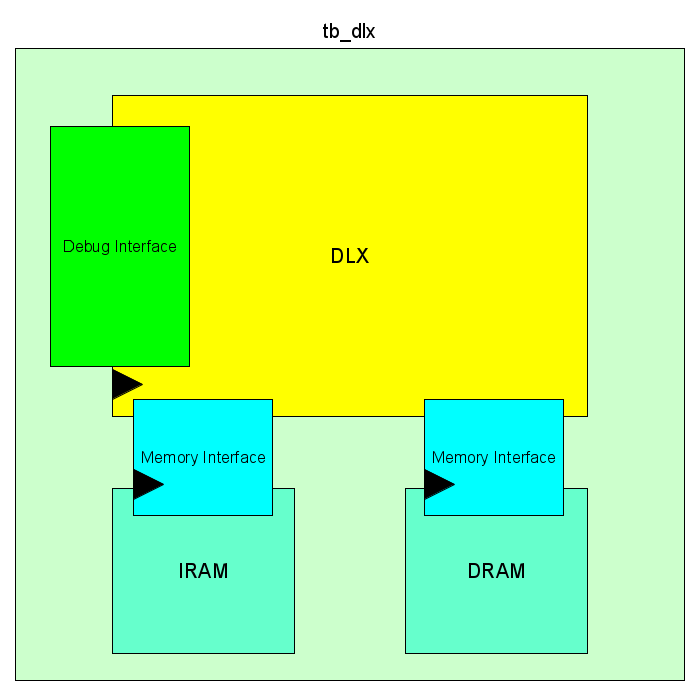
\includegraphics[scale=0.35,angle=0]{./chapters/figures/tb_dlx.png}
\caption{Testbench architecture}
\label{fig:tbdlx}
\end{figure}

In Figure \ref{fig:tbdlx} are missing the clock interconnections and the reset just for a matter of readability.\\ In this case :
\begin{itemize}
\item DLX, it is the microprocessor under test.
\item IRAM: it is the instruction ram which loads the program (compiled offline) for the unit under test.
\item DRAM: it is the data ram which loads at the beginning a file with random values and at every write operation it refreshes the content of another file.
\item Memory interface: it is the interface connecting the memories with the microprocessor. It has been defined as a single interface for both the memories, the only difference is in the modport configuration, where it can be distinguished between a read-only memory and a read-write memory (see Appendix \ref{appendix2}).
\item Debug interface: it is an interface that will be removed during the synthesis, its only purpose is to made visible the control signals of the CU in order to check if the instruction-dependent properties are covered (see Appendix \ref{appendix5}).
\end{itemize}

\subsection{Functional Coverage}
Functional coverage is a coverage metric defined to asses that the design has been adequately exercised\cite{paper:2}.
Observation points can be inserted at every granularity and in different points, external to the design (on the interfaces), inside the design or both of them.\\
As it can be seen in Figure \ref{fig:dlxtbcp} the observation point has been added on the interfaces, and they observe the read and write operation on memory as the memory address range(see Appendix \ref{appendix2}).

\begin{figure}[!htbp]
\centering
\captionsetup{justification=centering}
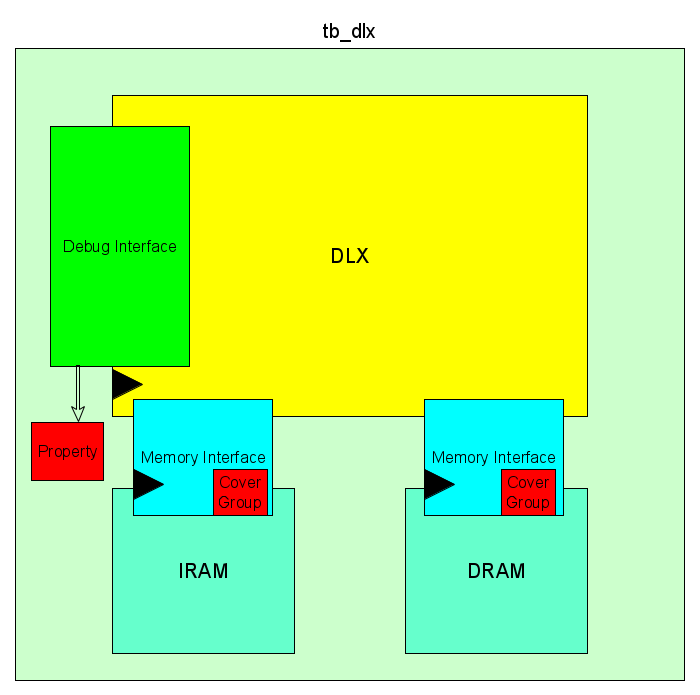
\includegraphics[scale=0.35,angle=0]{./chapters/figures/tb_dlx_cg.png}
\caption{Testbench architecture with coverpoint(in red)}
\label{fig:dlxtbcp}
\end{figure}
The covergroup is user-defined type which encapsulates the specifications of a coverage model which may include coverage points, points (signals) where values are sampled and stored in the internal database, Cross coverage between coverage points, triggering event for covergroup, other options to configure coverage object.\\
Instead of using covergroup, another approach is to reuse the property used for SVA. This approach has allowed to reuse the property defined for checking the correct behavior of the control unit, moving them outside the DLX and checking if those properties are covered by the Debug interface signals (which are the control signals from the control unit to the datapath). It is important to understand that the cover of those properties is program-dependent since they check the behavior for each type of instruction (r-type, i-type and j-type). Therefore, a test program able to test the whole ISA has been developed.\\\\
It is worth to mention that memories are never fully covered since their address range is very large, and they are exercised with test programs that use only a narrow subset of the memory range.

\newpage
\section{Universal Verification Methodology}
System Verilog has been developed as language that encapsulates the HDL and the HVL. Therefore, the usage of System Verilog as language for verification test benches has allowed to use a different architecture for functionally testing the DLX, the UVM approach.\\
The Universal Verification Methodology (UVM) is a standardized methodology for verifying integrated circuit designs\cite{paper:3}. UVM is derived mainly from the OVM (Open Verification Methodology). The UVM class library brings much automation to the SystemVerilog language such as sequences and data automation features (packing, copy, compare), and unlike the previous methodologies it is developed independently by the simulator vendors.\\
It exploits the OOP paradigm, therefore for each one of the entities that can be seen in Figure \ref{fig:tbuvm}, they represent a class with a specific function.

\begin{figure}[!htbp]
\centering
\captionsetup{justification=centering}
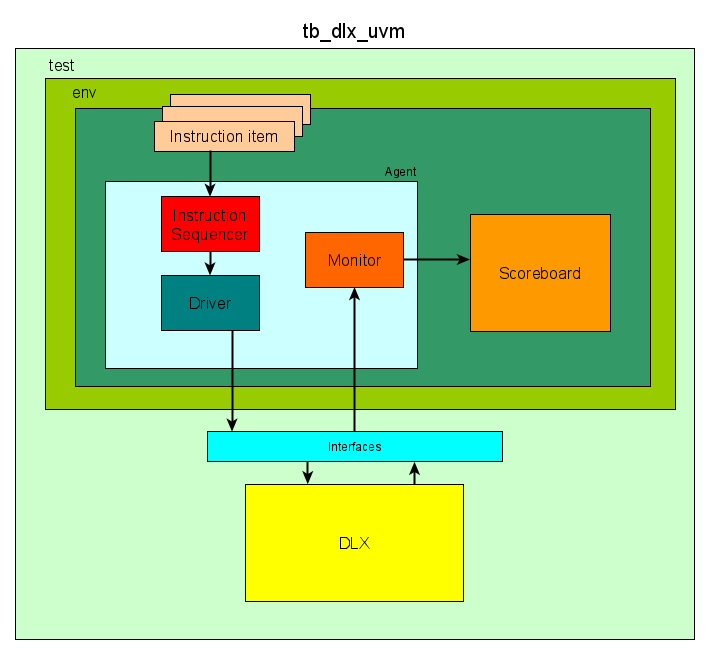
\includegraphics[scale=0.5,angle=0]{./chapters/figures/tb_dlx_uvm.png}
\caption{UVM testbench architecture}
\label{fig:tbuvm}
\end{figure}

Each class in Figure \ref{fig:tbuvm} inherits the functions and tasks of the relative UVM related class. For this specific case, the UVM classes function are (see Appendix \ref{appendix14}):
\begin{itemize}
\item Instruction item, it is the basic instruction for the microprocessor plus some additional function, such as its conversion to string, the retrieve of the only opcode and/or the opcode ALU function. It is important to mention that it includes the random variables for the opcode, opcode ALU function, r\textsubscript{d}, rs\textsubscript{1}, rs\textsubscript{2}, immediate and jump address(which are randomized when calling the relative function in instruction sequence) plus the constraint on the register, such as the one that the r\textsubscript{0} cannot be a destination register. Moreover, depending on the current opcode, it composes the instruction accordingly, i.e. the jump address is not needed when composing an add instruction and vice versa, even if all the variables are randomized every time.
\item Instruction sequence, it creates a given number of random instruction item.
\item Instruction sequencer, it only gives the instruction item from the instruction sequence to the driver one by one.
\item Driver, it retrieves the next instruction item from the sequencer and gives it to the DUV. It basically behaves as the IRAM of Figure \ref{fig:tbdlx}.
\item Monitor, this class is only in charge of sampling the Debug signals from the DUV and its current instruction.
\item Agent, since it is active it is in charge of creating the sequencer, driver and monitor classes and connects the driver port to the export port of the sequencer.
\item Scoreboard, it stores for each executed instruction if it passes the test or not and how many times it has been executed. It also checks if the correct signals(sampled from the Debug interface) have been asserted for the specific instruction. For example, \textit{add r\textsubscript{1}, r\textsubscript{3}, r\textsubscript{4}}, it will access to both the port of register file and then it will compute the addition between the accessed values and as last step it will write back the value in the register file. The scoreboard stores the signals from when the instruction is given to the microprocessor up to the 5-th clock cycle and then it compares the signals with an internal signature.
\item Environment, it instantiates the agent and the scoreboard and connects the analysis port of the scoreboard to the output port of the agent.
\item Test, it is only in charge of instantiate the environment class, it also applies a preliminary reset to all systems and then it creates the sequence of random instructions.
\item tb\_dlx\_uvm, it is the top level module which is in charge of instantiating the DUV, the interfaces. It interconnects the interfaces with DUV and starts the test (see Appendix \ref{appendix6}).
\end{itemize}